\documentclass[11pt]{exam}

\usepackage{amsmath}
\usepackage{graphicx}
\usepackage{geometry}
\usepackage{etoolbox}
\BeforeBeginEnvironment{choices}{\par\nopagebreak\minipage{\linewidth}}
\AfterEndEnvironment{choices}{\endminipage}
\geometry{
a4paper,
total={185mm,257mm},
left=10mm,
top=25mm,
bottom=10mm
}

\begin{document}
\setlength{\voffset}{-0.5in}
\setlength{\headsep}{5pt}

\fbox{\fbox{\parbox{8cm}{\centering
\vspace{2mm}
Testat - Versuch D - Zeitabhaengiger Strom - 2
\vspace{2mm}
}}}
\hspace{2mm}
\makebox[0.25\textwidth]{Name:\enspace\hrulefill} \hspace{5mm}
\makebox[0.2\textwidth]{Datum:\enspace\hrulefill}
\vspace{4mm}

\begin{questions}

\question Welche der folgenden Aussagen ist falsch?

\begin{choices}
	\choice Eine Wechselspannung wird durch Angabe der Signalform, Frequenz, Amplitude und Phase vollständig beschrieben.
	\choice Wenn die Spannung an einem Kondensator verdoppelt wird, verdoppelt sich auch die Kapazität. (correct)
	\choice Je größer der Widerstand in einem RC-Glied ist, desto größer ist die Zeitkonstante.
	\choice Je größer die Kapazität des Kondensators in einem RC-Glied ist, desto größer ist die Zeitkonstante.
	\choice Die Kapazität eines Kondensators trägt die Einheit Farad.
\end{choices}

\vspace{3mm}\question Ein zeitlich konstanter Strom \(\mathrm{I=100\,mA}\) fließt in einen Kondensator mit einer Kapazität von \(\mathrm{C=1\,mF}\) und lädt diesen auf. Wie groß ist die Spannung \(\mathrm{U}\) am Kondensator nach der Zeit \(\mathrm{t=100\,s}\)?\(\mathrm{Q=C \cdot U}\) und \(\mathrm{Ampere=Coulomb/Sekunde}\).

\begin{choices}
	\choice \(\mathrm{1000\,V}\)
	\choice \(\mathrm{10\,kV}\) (correct)
	\choice \(\mathrm{10\,V}\)
	\choice \(\mathrm{100\,kV}\)
	\choice \(\mathrm{100\,V}\)
\end{choices}

\vspace{3mm}\question Welche Frequenz hat das auf dem Oszilloskop gezeigte Signal? Der Skalierungsfaktor für die X-Achse beträgt \(\mathrm{0,5\,ms/DIV}\), der Skalierungsfaktor für die Y-Achse beträgt \(\mathrm{1\,V/DIV}\). 

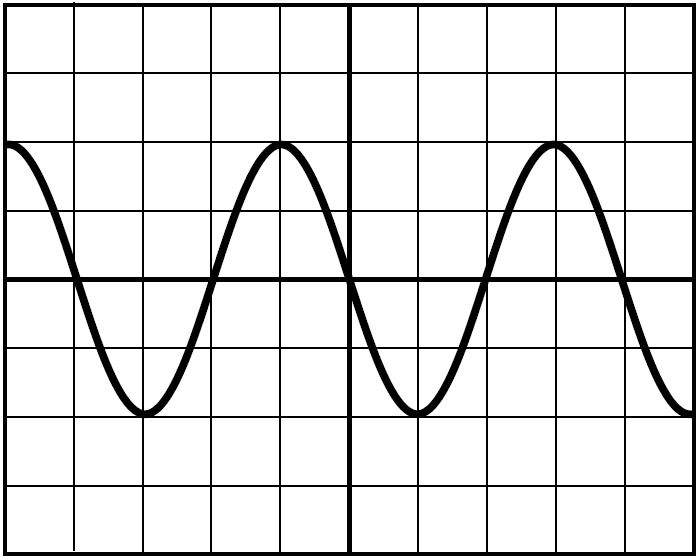
\includegraphics[width=0.5\textwidth]{../../../questions/D/images/Oszi1.png}

\begin{choices}
	\choice \(\mathrm{4\,ms}\)
	\choice \(\mathrm{250\,Hz}\)
	\choice \(\mathrm{500\,Hz}\) (correct)
	\choice \(\mathrm{1\,kHz}\)
	\choice \(\mathrm{2\,ms}\)
\end{choices}

\vspace{3mm}\question An einem Kondensator liegt eine Spannung von \(\mathrm{100\,kV}\) an. Er speichert dabei eine Ladung von \(\mathrm{100\,mC}\). Wie groß ist seine Kapazität?

\begin{choices}
	\choice \(\mathrm{10\,GF}\)
	\choice \(\mathrm{10\,kF}\)
	\choice \(\mathrm{1\,\mu F}\) (correct)
	\choice \(\mathrm{1\,F}\)
	\choice \(\mathrm{10\,\mu F}\)
\end{choices}

\vspace{3mm}\question Welcher der folgenden Kurvenverläufe gibt den Zusammenhang zwischen der angelegten Spannung und der Kapazität eines Kondensators qualitativ richtig wieder? 

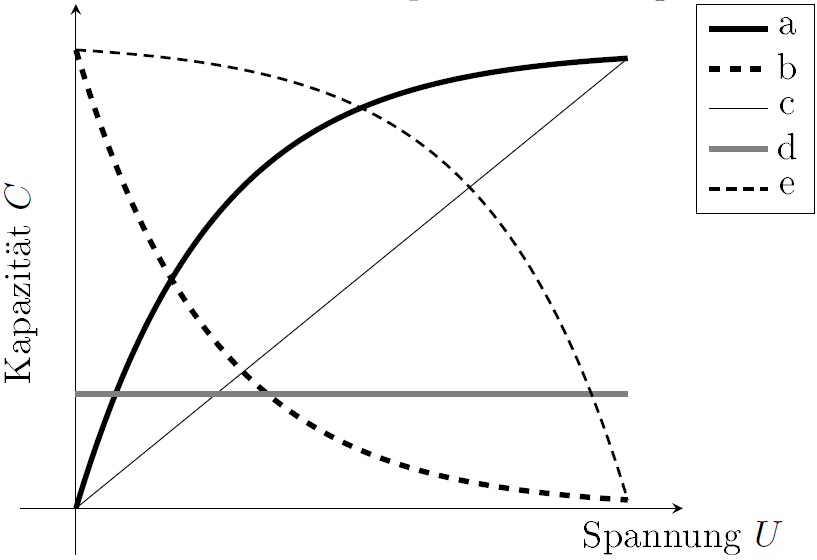
\includegraphics[width=0.5\textwidth]{../../../questions/D/images/Kondensator-C-U.png}

\begin{choices}
	\choice e
	\choice d (correct)
	\choice a
	\choice b
	\choice c
\end{choices}

\vspace{3mm}\end{questions}

\end{document}
